\documentclass[a4paper]{iacas}

\usepackage{cite}
\usepackage{hyperref}% embedding hyperlinks [must be loaded after dropping]
\usepackage{amsmath,amsthm,amssymb,amsfonts,latexsym,mathrsfs,wasysym}
\usepackage{marvosym}
\usepackage{subcaption}
\usepackage{soul,color}
\usepackage{threeparttable}% tables with footnotes
\usepackage{dcolumn}% decimal-aligned tabular math columns
\usepackage{float}
\usepackage{graphicx}
\usepackage{accents}
\usepackage{tikz}
\usepackage{lastpage}
\usepackage{fancyhdr}
\usepackage{color}
\usepackage{cancel}
\usepackage{setspace}
\usepackage{enumitem}
\usepackage{pdfpages}
\usepackage{algorithm}
\usepackage{algorithmic}
\usepackage{multirow}


%\doublespacing
% or:
\onehalfspacing
%\usepackage[T1]{fontenc}
%\usepackage{bigfoot} % to allow verbatim in footnote
\usepackage[framed,numbered]{matlab-prettifier}
\pagestyle{plain}
%\usepackage[hebrew,english]{babel}
\usetikzlibrary{shapes.geometric, arrows, calc}

\newcolumntype{d}{D{.}{.}{-1}}
\graphicspath{{figures/}}

% define some commands to maintain consistency
\newcommand{\pkg}[1]{\texttt{#1}}
\newcommand{\cls}[1]{\textsf{#1}}
\newcommand{\file}[1]{\texttt{#1}}
\newcommand{\sgn}[1]{\operatorname{sgn}\left(#1\right)}
\newcommand{\sat}[1]{\operatorname{sat}\left(#1\right)}
\newcommand{\rrule}[1]{\rule[#1]{0pt}{0pt}}
\newcommand{\fracds}[2]{\frac{\displaystyle #1\rrule{-0.2em}}{\displaystyle #2\rrule{1em}}}
\newcommand{\figref}[1]{Fig.~\ref{#1}}
\newcommand{\ubar}[1]{\underaccent{\bar}{#1}}
\newcommand{\norm}[1]{\lvert \lvert \vec #1 \rvert \rvert}

%diffeomorphism

\begin{document}

\begin{center}
 \large Image processing - 046200
 \end{center}
\begin{center}
\large\textbf{Homework \#3 wet}
 \end{center}


\begin{tabular}{l}
\\
{\bf\textit{Alexander Shender 328626114}} \\
{\bf\textit{Sahar Carmel 305554453}} \\
Technion - Israel Institute of Technology
\end{tabular}


\newpage
\section{Question 1}
The answers to the questions are the following: $R=2000$, $S = 8$.
\subsection{}
The $F_{1}$ function is the following:
\begin{equation*}
F_{1} = sin(2\pi(400/R)\cdot y) + sin(2\pi(50/R)\cdot x) + sin(2\pi(20/R)\cdot (x+y))
\end{equation*}
\subsection{}
The $F_{1}^{\Delta=1}$ was recreated using the above equation and we have received the result, identical to the one in the question. Size of the image: 200x200 px:

\vskip 0.1in
\begin{minipage}{0.5\textwidth}
\centering
	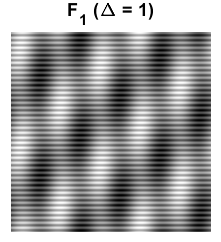
\includegraphics[scale=1]{imgs/q1_1.png}
\end{minipage}
\vskip 0.1in

\subsection{}
The 2D FFT was used to create the Fourier representation of the image. The Amplitudes are the following:

\vskip 0.1in
\begin{minipage}{0.5\textwidth}
	\centering
	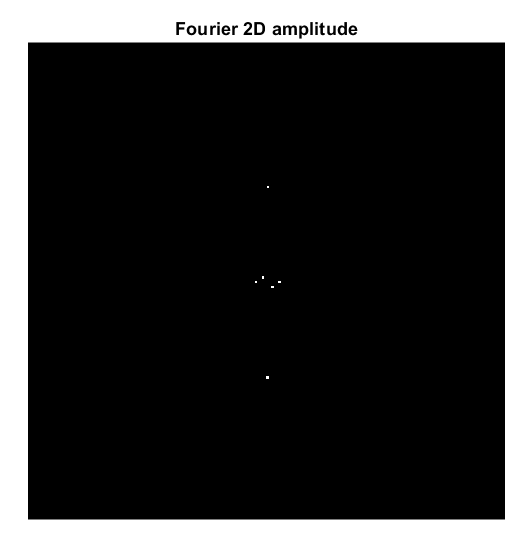
\includegraphics[scale=0.7]{imgs/q1_2.png}
\end{minipage}
\vskip 0.1in

As expected, we can see 6 deltas, according to the 3 frequencies that are present in the image:

\begin{enumerate}
\item Two dots on the vertical line $\rightarrow$ high frequency sine: $sin(2\pi(400/R)\cdot y)$
\item Two dots on the horizontal line $\rightarrow$ $sin(2\pi(50/R)\cdot x)$
\item Two dots on the diagonal line (smallest frequencies) $\rightarrow$ $sin(2\pi(20/R)\cdot (x+y))$
\end{enumerate}

To understand it easier, have colored those lines:

\vskip 0.1in
\begin{minipage}{0.5\textwidth}
\centering
	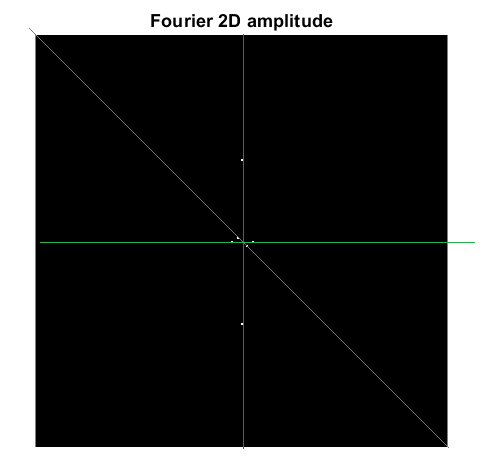
\includegraphics[scale=1]{imgs/q1_2_colored.png}
\end{minipage}
\vskip 0.1in

The exact coordinated of the deltas are:

% Please add the following required packages to your document preamble:
% \usepackage{multirow}
\begin{table}[]
\begin{tabular}{|c|c|c|c|}
\hline
                            & Row & Col & Distance from center (px) \\ \hline
Middle point                & 101 & 101 &                           \\ \hline
\multirow{2}{*}{ $sin(2\pi(400/R)\cdot y)$} & 61  & 101 & \multirow{2}{*}{40}       \\ \cline{2-3}
                            & 141 & 101 &                           \\ \hline
\multirow{2}{*}{$sin(2\pi(50/R)\cdot x)$}  & 101 & 96  & \multirow{2}{*}{5}        \\ \cline{2-3}
                            & 101 & 106 &                           \\ \hline
\multirow{2}{*}{$sin(2\pi(20/R)\cdot (x+y))$}  & 99  & 99  & \multirow{2}{*}{2.82}     \\ \cline{2-3}
                            & 103 & 103 &                           \\ \hline
\end{tabular}
\end{table}


\subsection{}
The image was not sampled with a sampling size ($\Delta$) of 9 $(S+1) = 8+1 = 9$. After performing the same procedure, the Fourier transform was found to give the following amplitures map:

\vskip 0.1in
\begin{minipage}{0.8\textwidth}
\centering
	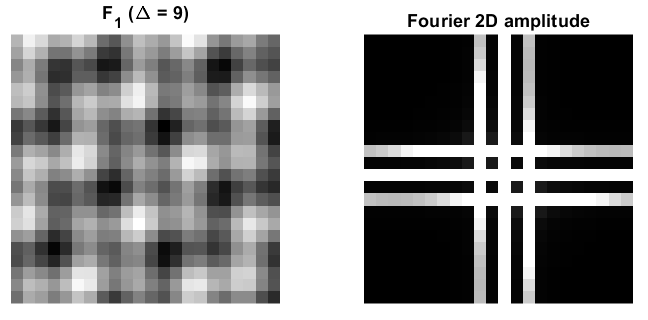
\includegraphics[scale=0.7]{imgs/q1_3.png}
\end{minipage}
\vskip 0.1in

We can clearly see the aliasing here. But the aliasing only occurs on the first 2 terms in $F_{1}$. 

%\begin{equation}
%\end{equation}



\subsection{}
A real image was taken, from the internet. The image contains various elements, windows at buildings, and other things which have high frequencies. Image was resized to 400x400 px. Plotting the image and its 2D FFT amplitudes gives:

\vskip 0.1in
\begin{minipage}{1\textwidth}
\centering
	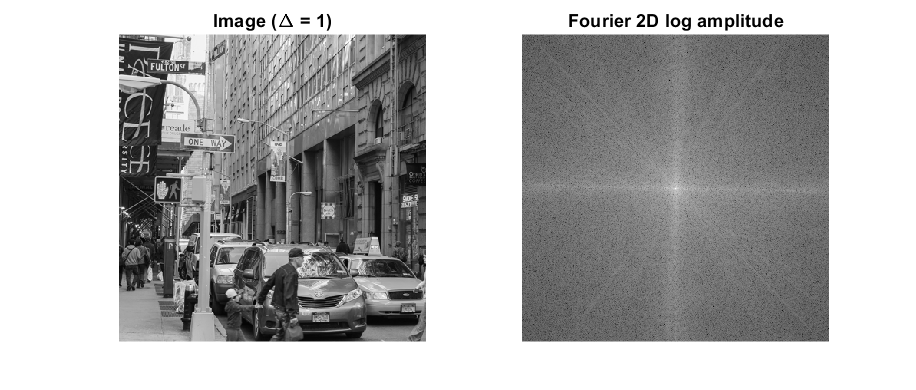
\includegraphics[scale=0.7]{imgs/q1_5.png}
\end{minipage}
\vskip 0.1in

\subsection{}
The sampling with the a sampling size of 4 was performed. The resulting image is of size 100x100 px. Plotting the image and its 2D FFT log amplitude. To answer the question, we plot the images together with the original image, for convenience.


\vskip 0.1in
\begin{minipage}{1\textwidth}
\centering
	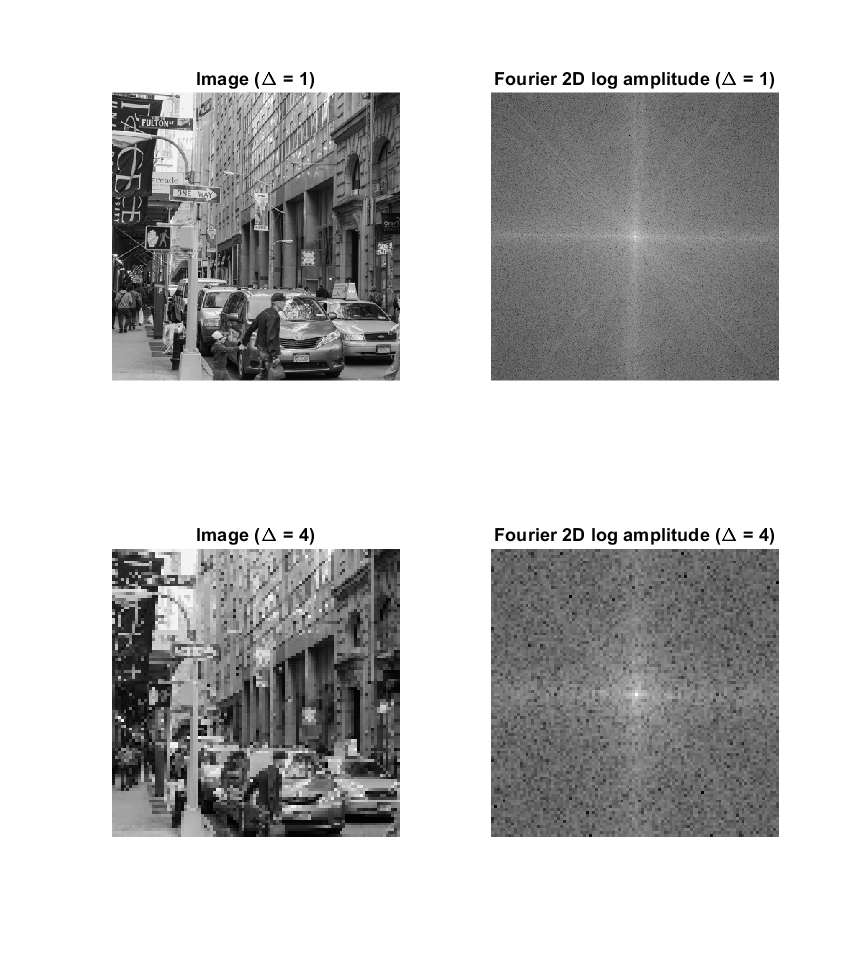
\includegraphics[scale=0.7]{imgs/q1_6.png}
\end{minipage}
\vskip 0.1in

Differences:
\begin{enumerate}
\item In spatial domain: we can see that the details that were small are not visible anymore, disappeared, because the sampling rate was too small to preserve them, and they got aliased with frequencies, which are smaller than Nyquist frequencies. Thus, those details are not visible anymore.
\item In frequency domain: We can see that the high frequencies got less intense, and most of them disappeared. We can see a shift towards the center of the frequencies plot, where the frequencies are lower. It happened because some high frequencies got aliased by the low frequencies, so their intensity rised.
\end{enumerate}

\subsection{}
In this subsection we first apply the Gaussian filter on the original image, and only then subsample. The results are the following:

\vskip 0.1in
\begin{minipage}{1\textwidth}
\centering
	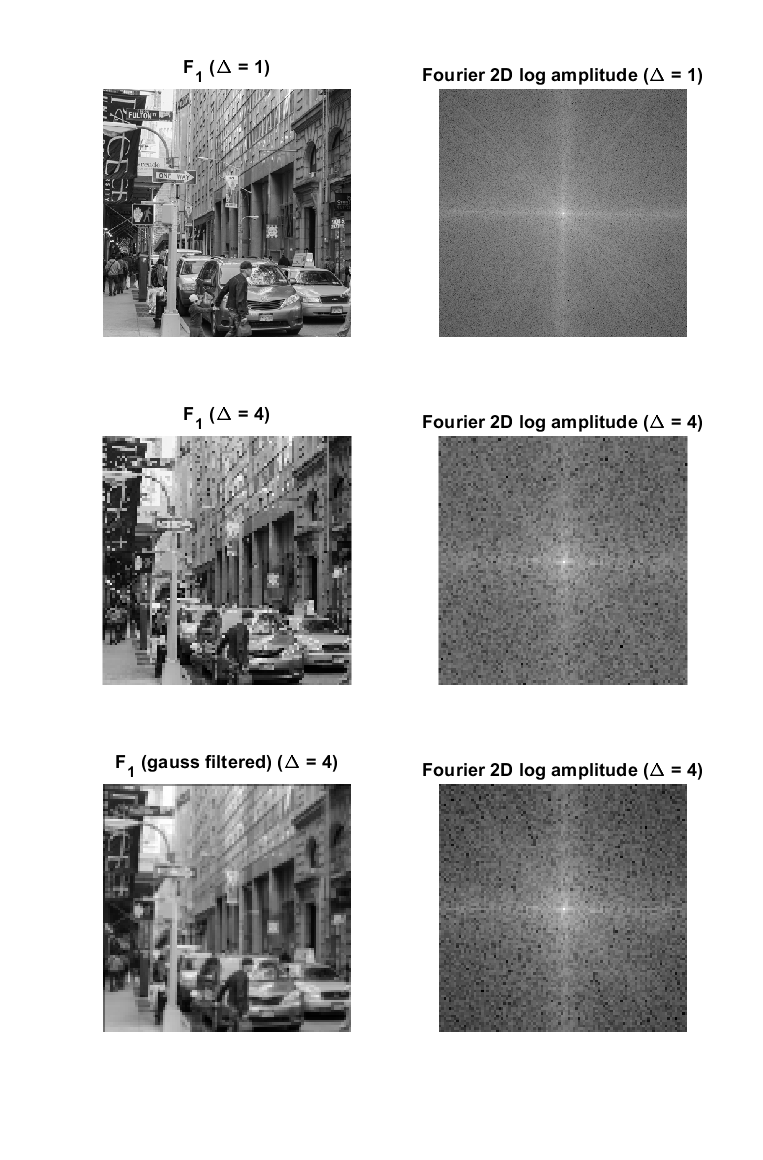
\includegraphics[scale=0.7]{imgs/q1_7.png}
\end{minipage}
\vskip 0.1in

We can observe that here, the high frequencies were better preverved! This is indeed one of the methods to reduce the aliasing effect. Because we have applied the Gaussian filter, the information of the image was better preserved, also on the pixels which were not sampled in the down-sampling process. 


\end{document}



















